\section{Matched Geometry and Pipeline Study}
\label{app:submissionstudy}

\begin{figure}[t]
 \centering
 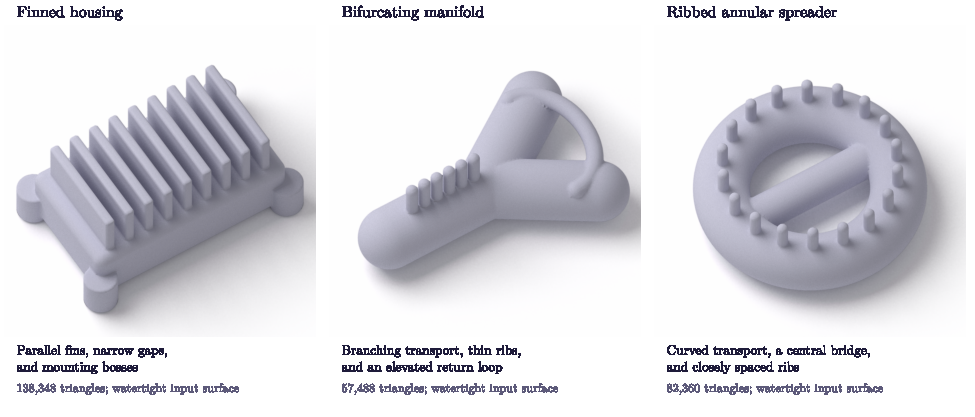
\includegraphics[width=\textwidth]{figures/submission-geometries.pdf}
 \caption{\textbf{Distinct application geometries.} Three watertight procedural
 test objects exercise different conduction paths and small geometric features.
 Every method uses the same surface, source configuration, and protected sensor
 within a case. Triangle count describes the input, not numerical difficulty.
 These are stylized conduction designs, not industrial cooling validations.}
 \label{fig:submissiongeometries}
\end{figure}

\subsection{A fixed-power, protected-region problem}
The additional study uses the same Poisson and ideal zero-Dirichlet cooling
model as the regional experiment, but replaces Gaussian source tails with
compact, fully protected heat components. This removes an ambiguity in the
fixed-count channel study: a lower objective can no longer result from deleting
a portion of a heat-generating source. All dimensions and temperatures are
nondimensional. No fluid or convective boundary model is implied.

For a center $c$, support radius $a>0$, and amplitude $A\geq0$, define
\[
 b_{c,a}(x)=\left(1-\frac{|x-c|^2}{a^2}\right)_+^2,
 \qquad f(x)=\sum_{j=1}^L A_j b_{c_j,a_j}(x).
\]
The sensor weight is $q=b_{s,b}/Q_b$, where $Q_b=32\pi b^3/105$.
The objective is $J(D)=\int_D q u_D\,dx$; the adjoint satisfies
$-\Delta p_D=q$ with homogeneous Dirichlet data. Component supports and the
sensor support are required to remain strictly inside the material.
The final protocol includes a low-power heat component of radius $0.085$
and amplitude $4$ at the protected sensor. This choice was fixed before the
measured campaign: an excluded remote-source-only pilot left the branching
sensor almost unheated and produced poorly resolved rare-event gradients.
The pilot is retained separately. Main heat sources remain stronger and
spatially distinct, so $f$ is not proportional to $q$.

\begin{proposition}[Exact normalization and preserved input power]
\label{prop:protectedpower}
Suppose $\overline{B_{a_j}(c_j)}\subset D$ for every $j$, and a removed set
$C$ is disjoint from these closed balls. Then
\[
 \int_{D\setminus\overline C} f\,dx
 =\int_D f\,dx
 =\sum_{j=1}^L\frac{32\pi A_j a_j^3}{105}.
\]
If $C$ also avoids $\overline{B_b(s)}$, then $\int_{D\setminus\overline C}q=1$.
For a point $X$ uniformly distributed in $B_b(s)$,
\[
 J(D)=\mathbb E\!\left[
 \frac{35}{8}\left(1-\frac{|X-s|^2}{b^2}\right)^2u_D(X)\right].
\]
\end{proposition}
\begin{proof}
\textbf{Step 1: restrict to the support.}
The positive-part definition makes $b_{c,a}$ zero outside $B_a(c)$.
Since this ball is contained in $D$ and untouched by $C$, its integral over
the original and the perforated domain is the same.
\textbf{Step 2: evaluate one radial integral.}
Translation and spherical coordinates give
\begin{align*}
 \int b_{c,a}(x)\,dx
 &=4\pi\int_0^a r^2(1-r^2/a^2)^2\,dr\\
 &=4\pi a^3\int_0^1(t^2-2t^4+t^6)\,dt\\
 &=4\pi a^3\left(\frac13-\frac25+\frac17\right)
 =\frac{32\pi a^3}{105}.
\end{align*}
\textbf{Step 3: sum the components.}
Linearity of the integral gives the displayed power identity. Disjointness
between heat components is unnecessary; only protection from removal is used.
\textbf{Step 4: normalize the sensor.}
Apply Step 2 with $(c,a)=(s,b)$ and divide by $Q_b$. Its support is unchanged,
so the integral of $q$ remains one.
\textbf{Step 5: express the objective as an expectation.}
The uniform-ball density is $1/V_b$ with $V_b=4\pi b^3/3$.
Consequently $\int q u=V_b\mathbb E[q(X)u(X)]$ and
$V_b/Q_b=35/8$, proving the formula. This identity concerns exact integrals;
finite quadrature and Monte Carlo estimates retain their numerical errors.
\end{proof}

\begin{proposition}[The local insertion coefficient for the new objective]
If a candidate $z$ lies outside all protected supports and satisfies the
regularity, separation, and cavity-expansion assumptions of the regional
result in \cref{app:regional}, then
\[
 \lim_{r\downarrow0}\frac{J(D\setminus\overline{B_r(z)})-J(D)}{4\pi r}
 =-u_D(z)p_D(z).
\]
\end{proposition}
\begin{proof}
\textbf{Step 1: identify the state and observation data.}
The compact bump and its first derivative vanish at its support boundary;
in particular the finite sums defining $f$ and $q$ are bounded and continuous.
The support-protection assumptions make both data independent of the inserted
cavity for all sufficiently small $r$.
\textbf{Step 2: specialize the regional objective.}
Its observation density is exactly the fixed, nonnegative $q$ above; the
adjoint is the solution of $-\Delta p=q$. The regional cavity expansion
therefore has coefficient $-u_D(z)p_D(z)$.
\textbf{Step 3: use the three-dimensional capacity convention.}
For the Laplacian convention used throughout the paper,
$\operatorname{cap}(B_r)=4\pi r$. Divide the expansion by this quantity and
let $r$ decrease to zero. The normalized remainder tends to zero under the
cited assumptions. This substitution provides no new remainder estimate,
and does not extend the separated-ball result to an overlapping channel.
\end{proof}

\subsection{Baselines and complete design costs}
Every pipeline starts from the same unperforated mesh, source configuration,
sensor, and paired candidate seed. We compare TWoS, deterministic multigrid
TD, deterministic hottest-point placement, and random placement of six
radius-$0.065$ spheres. The spheres remain disjoint and fully contained,
so every initialization and every subsequent translation removes exactly
$6(4\pi/3)(0.065)^3$ units of volume. Source and sensor clearance and a positive
inter-cavity gap are checked at every saved refinement state. Sphere centers
must remain at least $r+0.012$ from the outer boundary and at least
$r+a+0.018$ from each protected support center of radius $a$; pairs of
sphere centers must be separated by more than $2r+0.025$.

Each initialization is subsequently refined using our specialized implementation
of Differential WoS~\cite{miller2024differential}, Algorithm~2 and Eq.~(13).
For zero boundary data and inward offset $\ell$, a cavity-boundary hit contributes
$V_n\widehat u(x-\ell n)/\ell$ to the objective derivative; for a center
translation the parameter velocity has normal component $V_n=n\cdot v$.
The same radius, offset, gradient estimator, constraints, and backtracking
rule are used for all initializations. At each trial step, cavities are updated
in a cyclic order; each displacement is halved up to twelve times until feasible.
This avoids freezing all parameters when one cavity reaches a constraint. An
earlier global-rejection variant is retained as an excluded implementation
diagnostic; refinement and final evaluation were rerun for every method. TWoS and multigrid TD receive eight
refinement rounds; the hottest-point and random initializations additionally
receive rounds nine through sixteen. Independent evaluations at rounds
0, 4, 8, and, where applicable, 16 expose quality versus complete cost rather
than comparing only equal iteration counts. The two round allowances are not
identical wall-time budgets: distant initial cavities can produce few nonzero
boundary-gradient samples and consequently cheaper iterations. We therefore
report measured time explicitly and do not infer dominance at unmeasured budgets
or over all possible Differential WoS sampling schedules.

This is an attributed reimplementation of a paper component inside a common
benchmark, not the original authors' application optimizer. We checked the
terminal contribution and recursive boundary offset against the original authors' implementation. Differential WoS is not
in general restricted to topology-preserving changes. Here its fixed six-cavity
parameterization isolates initialization quality; this restriction is a choice
of comparison protocol, not a limitation claimed for that method.

TWoS uses 384 candidates, 48 scouting paths and 1,024 fresh rescore paths on
a 16-site shortlist per insertion. Multigrid solves for the primal and distinct
adjoint on a shared hierarchy with at most 65 nodes along the longest bounding-box
axis; other axis counts scale with the aspect ratio. It is our embedded Cartesian
finite-difference solver, not a finite-element implementation of another paper.
A separate complete-design baseline uses at most 49 nodes along the longest
axis with otherwise identical constraints and refinement. An additional
nearest-sensor control ranks candidates by Euclidean distance to the sensor
center and uses eight refinement rounds. It performs no PDE solve during
initialization, but shares every candidate and feasibility constraint. This
control tests whether simple proximity explains a benefit in the localized
observation task; it was added during the campaign as a baseline-strengthening
check, not selected through a parameter sweep. Independent resolution
checks use longest-axis counts 97 and 129. Convergence
to a $10^{-7}$ relative residual is checked separately from discretization error.

Complete design times include constructing the retained Embree geometry,
solver calls, request serialization, cavity selection, and all refinement or
radius-calibration decisions. Geometry generation, shared input preprocessing,
and independent evaluation are excluded. Backend high-water resident memory is
reported separately from driver memory. Instrumented outer-boundary distance
queries and parity rays are distinct counters; neither is inferred from the
number of walk steps. The measured campaign uses four OpenMP threads and single-threaded BLAS on
a Linux environment exposing an Intel Xeon Platinum 8573C, with an eight-CPU
quota and a 20 GiB memory limit. GCC 13.3 builds the C++17 backends with
\texttt{-O3}. Runs execute
serially without simultaneous rendering or other experiments. This is a
managed shared environment, not a dedicated timing node. The primary four
methods rotate order by seed; the two additional controls run subsequently,
so their timings should also be read in this execution context.

\paragraph{Guarded cavity offsets.}
A single ray-parity query can be ambiguous at a triangle edge. The following
geometric implication supplies a fallback specifically for contained spherical
cavities; it does not relax source protection or inter-cavity separation.

\begin{lemma}[An enclosing-ball test for a normal offset]
Let $D$ be open, $c\in D$, and $d=\operatorname{dist}(c,\partial D)>r+\ell$.
For any unit vector $e$, the point $c+(r+\ell)e$ belongs to $D$.
\end{lemma}
\begin{proof}
\textbf{Step 1: an open distance ball lies in the domain.}
If some $y$ with $|y-c|<d$ were outside $D$, the line segment from the
interior point $c$ to $y$ would first meet $\partial D$ at a point whose
distance from $c$ is at most $|y-c|<d$, a contradiction.
Thus $B_d(c)\subset D$.
\textbf{Step 2: apply the radius inequality.}
Since $|c+(r+\ell)e-c|=r+\ell<d$, this offset point belongs to $B_d(c)$,
and hence to $D$.
\end{proof}

The implementation retains its usual membership and analytic sphere-segment
checks. If the former rejects an offset, a positive enclosing-ball margin and
a checked interior cavity center provide an additional membership test. A
replay of the encountered case and an unchanged control are retained with
the benchmark. This is a numerical geometry guard under the stated mesh
assumptions, not a proof that floating-point distance and parity routines
are exact, and not the separate conservative application certificate.

\subsection{Finite-cavity estimator comparison}
Query timings use a retained outer-boundary acceleration structure, with
construction and an untimed warmup excluded for every estimator. Eight
protected, interior query sites are fixed per geometry before measuring
any estimator. A high-budget direct estimate uses sixteen independent batches
of 8,192 paths per site. Direct TWoS and common-random-number finite-cavity
differencing use sixteen repeats at 256 and 2,048 paths per site. For the latter,
the two state walks start at the same independently sampled sensor point and
use the same random stream in the original and perforated domain. Their
weighted difference is divided by $4\pi r$. Trial radii are
$0.08,0.04,0.02,0.01$. This is a specified local coupling, not a claim that
all possible finite-difference couplings have been optimized.

We additionally evaluate a stronger stopped-path baseline. It estimates the
finite cavity correction directly, rather than subtracting two noisy source
integrals. The following identity specifies precisely which quantity it estimates.

\begin{proposition}[A finite-cavity harmonic-correction estimator]
Let $D$ be bounded and let $D_r=D\setminus\overline{B_r(z)}$, with the cavity strictly contained and
disjoint from the sensor support. Let $u_D$ and $u_{D_r}$ solve the same Poisson equation $-\Delta u=f$ on their respective domains with zero Dirichlet data. Assume the domains are regular for the
Dirichlet problem and the state solutions are continuous up to their boundaries.
Let $Y$ be uniform in $B_b(s)$, let $X$ be a Brownian path started at $Y$, and
let $\tau_r$ be its first exit from $D_r$. Write
$W(Y)=(35/8)(1-|Y-s|^2/b^2)^2$ and
$H_r=\{X_{\tau_r}\in\partial B_r(z)\}$. Suppose $U_0(x)$ is a conditionally
unbiased, independent estimate of the original-domain temperature $u_D(x)$.
Then
\[
 Z_r=\frac{W(Y)\,\mathbf1_{H_r}\,U_0(X_{\tau_r})}{4\pi r}
 \quad\hbox{satisfies}\quad
 \mathbb E Z_r=\frac{J(D)-J(D_r)}{4\pi r}.
\]
The statement assumes the displayed expectation is integrable. Exact paths and
conditionally unbiased state estimates are mathematical assumptions here;
finite-termination implementations retain their numerical errors.
\end{proposition}
\begin{proof}
\textbf{Step 1: subtract the two PDEs.}
On $D_r$, both states have the same source, so $h=u_D-u_{D_r}$ satisfies
$-\Delta h=0$. On the old boundary, both states vanish and hence $h=0$.
On the cavity boundary, $u_{D_r}=0$ and hence $h=u_D$.
\textbf{Step 2: derive the harmonic exit representation.}
Fix $y\in D_r$. The difference $h$ is harmonic in $D_r$ and continuous on its
compact closure, hence bounded. Localize the Brownian motion to compact
interior subdomains and a finite time $t$. It\^o's formula for the localized
process has drift $(1/2)\Delta h=0$; its stochastic integral has zero mean
because the localized derivatives are bounded. Thus the expectation of the
stopped $h$ remains $h(y)$. Exhausting the domain gives the same equality
for $h(X_{t\wedge\tau_r})$ by dominated convergence. The exit time $\tau_r$
is finite almost surely: $D_r$ is contained in a ball, whose Brownian exit
time has finite expectation, and exiting $D_r$ occurs no later than exiting
that ball. Letting $t\to\infty$ and using boundedness and boundary continuity
therefore yields
\[
 h(y)=\mathbb E_y[h(X_{\tau_r})]
     =\mathbb E_y[\mathbf1_{H_r}u_D(X_{\tau_r})].
\]
The second equality uses exactly the two boundary values from Step 1;
it introduces no source-integral subtraction.
\textbf{Step 3: replace the boundary temperature by a fresh estimate.}
Condition on $Y$, the entire exit path, and its terminal point. Conditional
unbiasedness of the independent nested estimate gives
$\mathbb E[U_0(X_{\tau_r})\mid Y,X]=u_D(X_{\tau_r})$.
Applying the tower property therefore leaves the expression in Step 2 unchanged.
\textbf{Step 4: integrate the protected observation.}
The cavity does not remove any sensor weight. Proposition~\ref{prop:protectedpower}
and the tower property give
$\mathbb E[W(Y)h(Y)]=\int q(u_D-u_{D_r})=J(D)-J(D_r)$.
\textbf{Step 5: normalize.}
Divide this equality by $4\pi r>0$. The result is a finite-radius difference;
identifying its limit with $u_D(z)p_D(z)$ still requires the separate cavity
asymptotics. No finite-radius equality with that point product has been asserted.
\end{proof}

The implementation uses a perforated-domain boundary walk followed by one
independent original-domain source walk only on a new-cavity hit. It reports
the number of such hits, distance queries, time, and estimator variance. This
baseline tests the rare-event mechanism after removing unnecessary subtraction
noise. The common-random-number subtraction baseline is retained as a separate
implementation, rather than conflating the two couplings.

Variance about each estimator's own mean is kept separate from RMS error to
the high-budget infinitesimal reference. A finite-radius difference has a
different expectation from a topological derivative; its error includes this
remainder as well as sampling and termination error. The reference also has
sampling and termination error and is not labeled ground truth. Aggregate
errors weight high-influence sites more strongly; a reference with no sampled
contribution at a remote site does not establish a zero exact coefficient.
The data release reports reference standard error and the number of zero
reference estimates. A degenerate bootstrap interval from zero observed hits
likewise does not establish zero population variance. Multigrid
query estimates use longest-axis counts 49, 65, 97, and 129. Additional finite-hole
resolution checks explicitly expose grid differences that fail to resolve
the smallest cavities; a small linear-solver residual cannot resolve that issue.

\subsection{Matched finite channels}
Each channel is the union of balls at spacing $0.04$ along a vertical axis,
with centers from $z=-0.48$ to $0.80$. These endpoints lie beyond every
geometry's vertical bounds. For radius $r>0.02$, \cref{prop:channelcore} gives
a positive core radius $\sqrt{r^2-0.02^2}$. Parallel axes protect all compact
sources and the sensor by \cref{prop:channelprotection}. The shared candidate
pool is conservatively generated with maximum radius $0.11$, including the
source-clearance and axis-separation tests, even though calibrated radii are
usually smaller. This restriction is common to every method; the experiment
does not optimize over all feasible channel locations at the final radius.

After the $k$th axis is selected, a shared common radius is calibrated to
removed volume $0.0028k$ using a fixed scrambled Sobol sample of $2^{20}$
bounding-box points. Recalibration can change previous channels. Four independent
$2^{20}$-point scrambles audit the final volume; their dispersion is a numerical
integration diagnostic, not a certified enclosure. Six channels target total
volume $0.0168$. Neither equal radii nor equal channel counts are used as a
substitute for the volume measurement. The axis-point topological score remains
a heuristic for a finite channel, followed by independent objective evaluation.

\subsection{Evaluation, geometry, and visualization}
Five paired seeds are used on a finned housing, a bifurcating manifold with
thin ribs and an elevated return loop, and a ribbed annular spreader with a
central bridge. They are procedural application test objects, not standardized
industrial datasets. The latter two test branching and curved transport in
addition to the housing's narrow gaps and extended fins; surface triangle count
alone is not treated as evidence of numerical difficulty.

Each saved objective is evaluated in four independent scrambled-Sobol sensor
blocks of 128 points with 512 walks per point. The exact weight in
\cref{prop:protectedpower} is used. Paired-seed summaries retain the variation
between designs and separately report evaluation-block uncertainty. Additional
paired intervals jointly bootstrap the five design seeds and the four evaluation
blocks; block resampling is shared across methods and seeds to preserve the
common-random-number dependence. These are approximate, small-sample intervals,
not certified coverage guarantees. Reusing
the same evaluation blocks across methods supports paired differences; those
blocks never participate in candidate selection or line-search acceptance.
The housing-channel comparison exposed several percentage points of disagreement
between independent numerical references. We therefore added a uniform refinement
rule: a first-seed case is reevaluated at longest-axis counts 193 and 257 if any
method changes by more than 1 percentage point from grid 97 to 129 or differs
by more than 2 points between Monte Carlo and grid 129. Every method in a flagged
case is checked. This rule was introduced during reference auditing, rather than
claimed as a preregistered test; the added solves are excluded from design times.
Line search itself is heuristic and is not reported as certified.

\paragraph{Uncertainty bands and bars.}
Let $J_{m,k,b}$ be the independently evaluated objective for method $m$,
design seed $k\in\{1,\ldots,5\}$, and evaluation block
$b\in\{1,\ldots,4\}$, and let $J_{0,k,b}$ denote its unperforated reference.
The reported mean reduction is
\[
 \overline R_m=\frac15\sum_{k=1}^5
 100\left(1-\frac{\sum_b J_{m,k,b}}{\sum_b J_{0,k,b}}\right).
\]
For each of 4,000 bootstrap replicates, we resample five seed indices and four
block indices with replacement, then recompute this expression. The same indices
are used across methods and checkpoints, retaining the paired design and
common-random-number structure. Shaded trajectory bands are the pointwise
2.5th and 97.5th percentiles. Isolated channel results use vertical bars instead.
Horizontal bars resample measured complete-design times over the same seed
indices; they include both algorithmic and machine-timing variation. Faint
points show the individual design runs. Bands between checkpoints are visual
interpolation, not evaluations at every intervening time or simultaneous
confidence regions for an entire optimization path.

For an estimator setting, let $S_i\in\mathbb R^8$ be its vector of scores in
repeat $i$, and let $T_j\in\mathbb R^8$ be one of sixteen high-budget reference
batches. With $\overline T=16^{-1}\sum_jT_j$, the displayed relative variance
and RMS error are respectively
\[
 V=\frac{\sum_{a=1}^8\widehat{\operatorname{Var}}_i(S_{i,a})}
         {\|\overline T\|_2^2},\qquad
 E=\sqrt{\frac{\frac1n\sum_{i=1}^n\|S_i-\overline T\|_2^2}
                    {\|\overline T\|_2^2}}.
\]
We independently resample the sixteen repeat vectors and sixteen reference
batches 4,000 times. Sites remain together within each vector; treating sites as
independent experimental replicates would be inappropriate. Percentile bands
around $V$ measure uncertainty in the estimated variance, not the standard
deviation of an individual score. RMS-error bars additionally reflect sampling
uncertainty in the reference. A deterministic multigrid setting has one output:
its error bar reflects only reference sampling, and no Monte Carlo field variance is inferred. Timing intervals use five
additional repetitions per grid with rotated resolution order and a retained
outer mesh; each call rebuilds its multigrid hierarchy. All repeated fields
are checked against the original deterministic output. For the eight-site
query benchmark, a scheduling audit found that the original dynamic chunk of
four exposed only two work chunks to four threads. We repeat the direct-score
timing with chunk size one, verify every score and component field bitwise
against the retained original output, and use these repeats for query-time
plots. Original timings remain in the raw records. This correction changes
neither the numerical samples nor the recorded complete-design timings, which
retain their original scheduling. Numerical discretization, termination, offset,
and finite-radius bias are not enclosed by these bootstrap intervals. With only
five design seeds and sixteen estimator repeats, the intervals remain
approximate descriptive evidence, not established frequentist coverage or a
finite-insertion certificate. In particular, resampling cannot reveal rare
events absent from the recorded repeats; a zero observed score does not
establish zero temperature or influence. Site-level raw scores and cavity-hit
counts are retained for this reason. When all recorded correction vectors
are zero, we report the empirical output but suppress collapsed variance and
RMS-error intervals and mark variance unresolved. The earlier Bunny allocation bands in
\cref{fig:teaser,fig:bunnybudget} remain observed ranges over three designs;
they are not relabeled as confidence intervals.

Figures use the first predetermined seed, rather than selecting the visually
best design. Camera, section plane, display window, lighting, and map scale
are held fixed within each geometry. The local cooling map displays
$1-u_D(x)/u_{D_0}(x)$ on the visible material section using a longest-axis-193
multigrid field, clipped to $[0,1]$ for display. Material is gray where the
unperforated section temperature is below $10^{-4}$ of its maximum, avoiding
misleading relative changes in essentially cold material. Quantitative objective values
come from the separate evaluations above. A faint depth-tested shell shows
the physically present upper structure removed only for presentation.
The display cut, tessellated cavity surfaces, and lighting denoiser never enter
the PDE or its objective. Section colors are applied from the interpolated numerical field after
radiance denoising.

\begin{figure}[t]
 \centering
 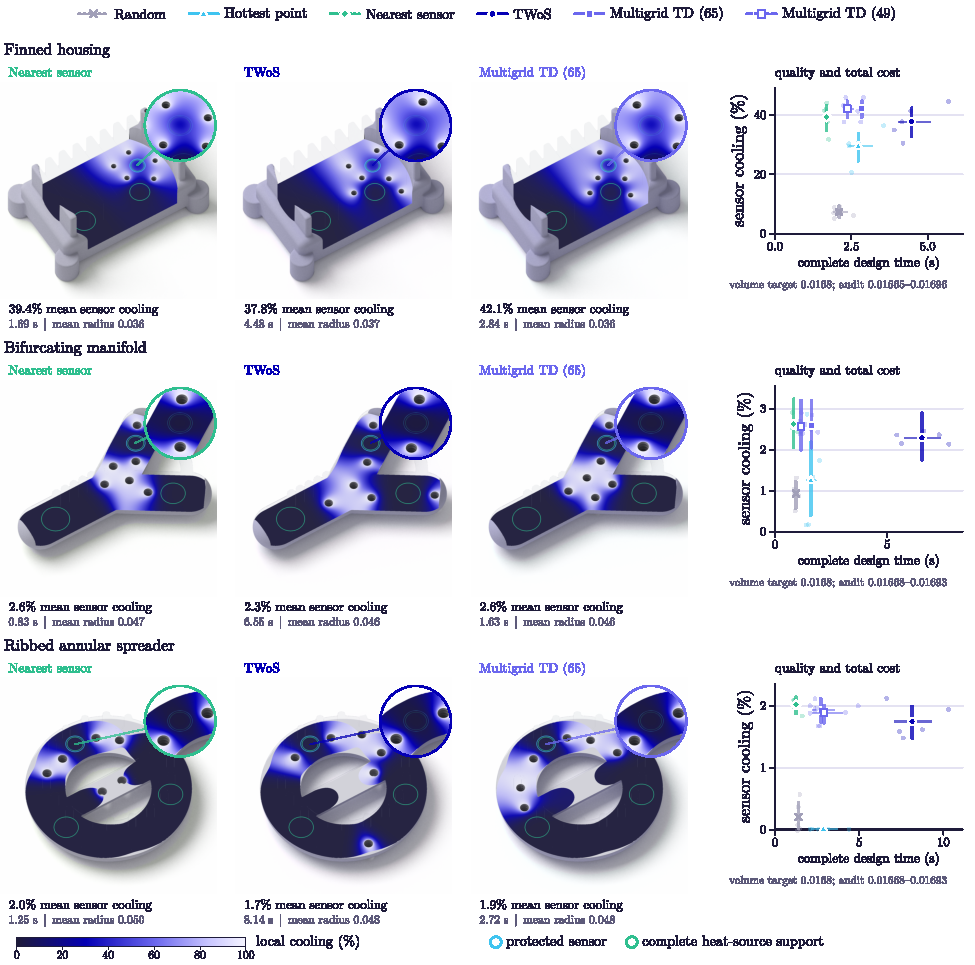
\includegraphics[width=\textwidth]{figures/submission-channels.pdf}
 \caption{\textbf{Accessible designs with controlled material and power budgets.}
 Six open ball-union channels are selected under identical source and sensor
 protection constraints. A common radius is calibrated to total removed volume
 $0.0168$; the displayed audit range spans the independent mean volume estimates
 over all methods and seeds in each geometry, not a certified interval.
 Heat input is exactly invariant under the protected-support model.
 Views use the first predeclared seed; quantitative summaries use five seeds.
 Vertical bars give pointwise 95\% bootstrap intervals for mean cooling,
 resampling seeds and independent evaluation blocks together across methods.
 Horizontal bars describe uncertainty in mean runtime across seeds; plot
 ranges adapt to each geometry while retaining the same physical units.
 The local cooling field shares a scale across designs. No coolant flow is
 solved, and the point score remains a heuristic for these extended removals.}
 \label{fig:submissionchannels}
\end{figure}


